\documentclass[11pt]{article}

% ============================================================================
%  Dobbertin Theorem 1 -- equation (1) and the step (1) => (2)
%  A paper-to-Lean map, presented in the topological order of the Lean library
%  (from the Mathlib foundations up to the headline results).
% ============================================================================

\usepackage[a4paper,margin=2.3cm]{geometry}
\usepackage{amsmath,amssymb,amsthm}
\usepackage{xcolor}
\usepackage{framed}
\usepackage{listings}
\usepackage{tikz}
\usetikzlibrary{arrows.meta,positioning,shapes.geometric,fit,backgrounds,calc,shapes.multipart}
\usepackage{tikz-cd}
\usepackage{enumitem}
\usepackage[hidelinks]{hyperref}
\usepackage{caption}
\usepackage{fontspec}
\setmonofont{DejaVu Sans Mono}

% ---------------------------------------------------------------------------
%  Colours
% ---------------------------------------------------------------------------
\definecolor{leanbg}{RGB}{245,247,250}
\definecolor{leanframe}{RGB}{200,210,222}
\definecolor{leankw}{RGB}{150,20,120}
\definecolor{leancmt}{RGB}{90,120,90}
\definecolor{leanstr}{RGB}{160,80,20}
\definecolor{quotebar}{RGB}{40,90,160}
\definecolor{mathlibcol}{RGB}{215,232,255}
\definecolor{defscol}{RGB}{222,245,222}
\definecolor{enginecol}{RGB}{255,244,214}
\definecolor{headcol}{RGB}{255,224,224}
\definecolor{bridgecol}{RGB}{235,225,255}

% ---------------------------------------------------------------------------
%  Lean listing style with a literate map for the Unicode used in the sources
% ---------------------------------------------------------------------------
\lstdefinelanguage{lean4}{
  morekeywords={theorem,lemma,def,noncomputable,variable,namespace,end,open,
    import,scoped,in,by,fun,if,then,else,do,with,match,let,have,show,from,
    calc,intro,intros,exact,apply,rw,rwa,simp,simp_all,ring,ring_nf,omega,
    omit,convert,using,refine,refine',obtain,rcases,rintro,constructor,funext,
    set,unfold,cases,induction,at,Prop,Type,Function,structure,instance,
    grind,decide,linarith,nlinarith,linear_combination,field_simp,aesop,
    tauto,by_contra,exfalso,contrapose,use},
  sensitive=true,
  morecomment=[l]{--},
  morecomment=[s]{/-}{-/},
  morestring=[b]",
}

\lstset{
  language=lean4,
  basicstyle=\ttfamily\footnotesize,
  keywordstyle=\color{leankw}\bfseries,
  commentstyle=\color{leancmt}\itshape,
  stringstyle=\color{leanstr},
  backgroundcolor=\color{leanbg},
  frame=single,
  rulecolor=\color{leanframe},
  framesep=5pt,
  xleftmargin=6pt,
  xrightmargin=2pt,
  breaklines=true,
  breakatwhitespace=false,
  columns=fullflexible,
  keepspaces=true,
  showstringspaces=false,
}

% inline Lean (works in text, math, tikz-cd, and moving args)
\protected\def\lc#1{\texttt{\detokenize{#1}}}

% ---------------------------------------------------------------------------
%  Paper-quote environment
% ---------------------------------------------------------------------------
\newenvironment{paperquote}[1]
 {\par\smallskip\noindent
  \def\FrameCommand{\color{quotebar}\vrule width 3pt\hspace{8pt}}%
  \MakeFramed{\advance\hsize-\width \FrameRestore}%
  \small\itshape
  \noindent\normalfont\footnotesize\textbf{\textsf{Dobbertin (1999) --- #1}}\par\nobreak\smallskip\itshape}
 {\endMakeFramed\par\smallskip}

% ---------------------------------------------------------------------------
%  Theorem-like
% ---------------------------------------------------------------------------
\theoremstyle{definition}
\newtheorem{correction}{Correction}
\newtheorem*{remark}{Remark}

\title{\textbf{Dobbertin's Theorem 1 --- Equation (1) and the step (1)\,$\Rightarrow$\,(2)}\\[4pt]
\large A paper-to-Lean\,4 map, in the topological order of the formalisation\\[2pt]
\normalsize from the Mathlib foundations to the headline results}
\author{Formalisation library \texttt{Dobbertin1999MVP.Equation1.*}}
\date{}

\begin{document}
\maketitle

\begin{abstract}
\noindent
This document places, \emph{side by side}, the relevant passages of
H.~Dobbertin, \emph{Kasami Power Functions, Permutation Polynomials and Cyclic
Difference Sets} (1999, pp.~133--138) and their Lean\,4 formalisation in the
\texttt{Dobbertin1999MVP.Equation1.*} library.  The material is ordered
\emph{exactly as the Lean library is built} --- i.e.\ along a topological sort
of the module dependency DAG, from the Mathlib foundations at the bottom up to
the headline results \lc{theorem_1}, \lc{eqn2_of_eqn1} (the step (1)\,$\Rightarrow$\,(2))
and the two case analyses.  Each layer is accompanied by TikZ dependency
diagrams and \texttt{tikz-cd} commutative diagrams visualising how the paper's
argument is threaded through the Lean declarations.  Every declaration quoted
here is \texttt{sorry}-free in the sources and, as recorded in the project's
architecture report, rests only on the standard axioms \lc{propext},
\lc{Classical.choice}, \lc{Quot.sound}.
\end{abstract}

\tableofcontents
\bigskip

% ===========================================================================
\section{How to read this document}
% ===========================================================================

The library is a self-contained extract carrying exactly the material needed,
end to end from \texttt{Mathlib}, for \textbf{equation (1)} of Theorem~1 and its
first substantive step $(1)\Rightarrow(2)$.  Equation~(1) is the equation
$q_\alpha(x)=c$ cleared of denominators,
\[
   c\,x^{2^k+1} \;=\; \sum_{i=1}^{k'} x^{2^{ik}} \;+\; \alpha\,\mathrm{Tr}(x).
   \tag{1}
\]

The exposition follows the \emph{compile order} of the library.  Concretely, a
Lean file may only refer to declarations that appear earlier in the dependency
DAG, so reading the modules in topological order is the same as reading the
mathematics ``from the foundations up''.  We use two visually distinct blocks:

\begin{itemize}[nosep]
  \item a blue-barred \emph{paper quote} block for passages of Dobbertin (1999); and
  \item a boxed Lean listing for the corresponding formalisation.
\end{itemize}

\noindent
The global correspondence is summarised in Table~\ref{tab:map}.

\begin{table}[h]
\centering
\captionsetup{font=small}
\caption{Paper object $\leftrightarrow$ Lean declaration (headline thread).}
\label{tab:map}
\small
\begin{tabular}{@{}p{0.50\linewidth}p{0.30\linewidth}p{0.12\linewidth}@{}}
\hline
\textbf{Paper object} & \textbf{Lean (\lc{Dobbertin1999.Paper})} & \textbf{status}\\
\hline
Trace $\mathrm{Tr}(x)=\sum_{i<n}x^{2^i}$ & \lc{def Tr} & def\\
Generalized Kasami poly.\ $q_\alpha$ & \lc{def qKasami} & def\\
Equation (1) & \lc{def eqn1} & def\\
$\ell(x)=c^{2^k}x^{2^{2k}}+x^{2^k}+cx+1$ & \lc{def ell} & def\\
$(2^k-1)^{-1}\ (\mathrm{mod}\ 2^n-1)$ exists & \lc{inv_mod_exists} & \checkmark\\
``only if'' at $q_\alpha(1)$ & \lc{qKasami_one_eq_zero_iff} & \checkmark\\
Theorem 1 (permutation criterion) & \lc{theorem_1} & \checkmark\\
\textbf{Step (1) $\Rightarrow$ (2)} & \lc{eqn2_of_eqn1} & \checkmark\\
Case 1 (unique root of $\ell$) & \lc{theorem_1_case1} & \checkmark\\
Case 2 factorisation $\ell=Q^{2^k}+fQ$ & \lc{ell_eq_Q} & \checkmark\\
Case 2 (unique nonzero solution of (1)) & \lc{theorem_1_case2} & \checkmark\\
\hline
\end{tabular}
\end{table}

% ===========================================================================
\section{The dependency DAG (Mathlib $\to$ headlines)}
% ===========================================================================

The library is eight modules in four layers.  Figure~\ref{fig:dag} is the full
module dependency graph; arrows are \lc{import}/\emph{uses} edges and point in
the direction of dependence (a module points to the modules it is built on).
Reading the figure \emph{bottom-to-top} is the topological order used by the
rest of this document.

\begin{figure}[h]
\centering
\resizebox{\textwidth}{!}{%
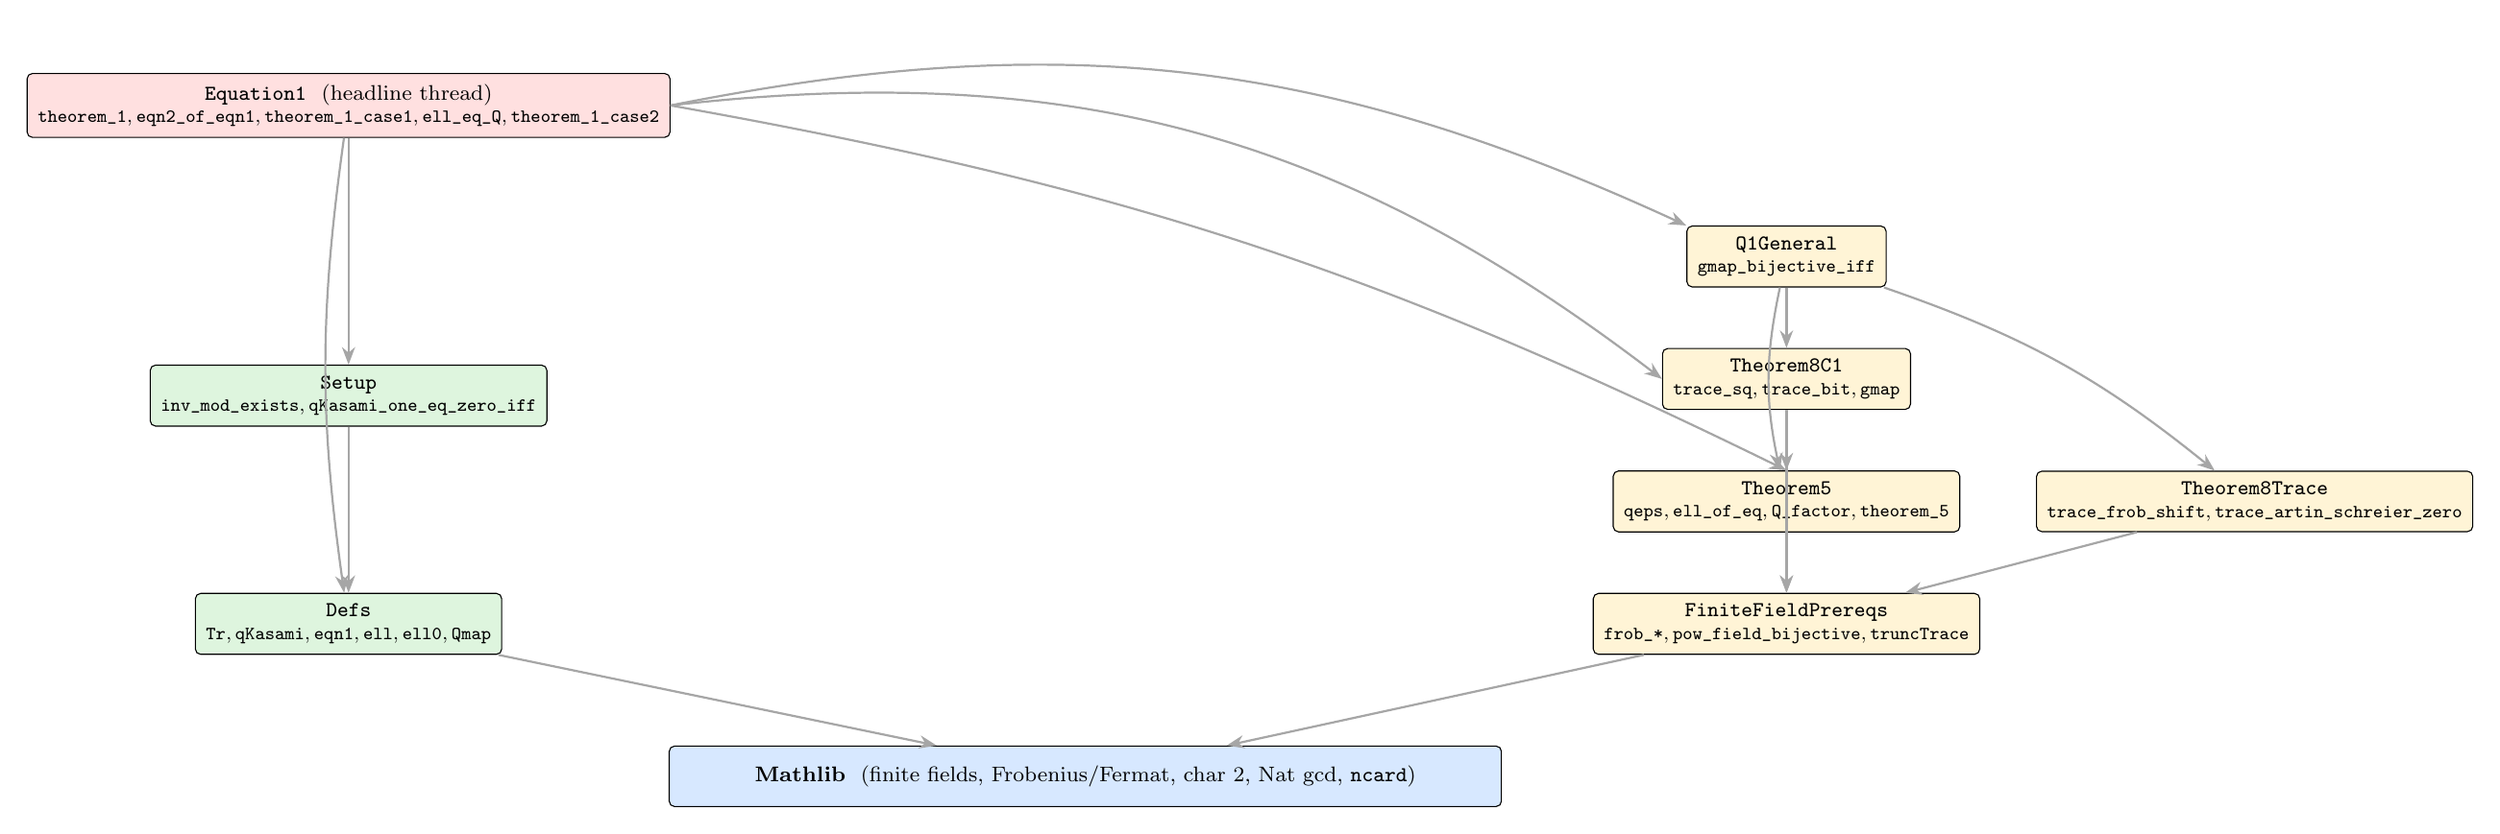
\begin{tikzpicture}[
   >=Stealth, node distance=6mm,
   box/.style={draw, rounded corners=2pt, align=center, font=\footnotesize,
               inner sep=4pt, minimum height=8mm},
   dep/.style={->, thick, gray!70},
]
% layer 0
\node[box, fill=mathlibcol, minimum width=11cm] (ml)
  {\textbf{Mathlib}\ \ \footnotesize (finite fields, Frobenius/Fermat, char 2,
   Nat gcd, \lc{ncard})};
% layer 1
\node[box, fill=defscol, above left=12mm and 2.2cm of ml] (defs)
  {\lc{Defs}\\[-1pt]\scriptsize \lc{Tr},\,\lc{qKasami},\,\lc{eqn1},\,\lc{ell},\,\lc{ell0},\,\lc{Qmap}};
\node[box, fill=enginecol, above right=12mm and 1.2cm of ml] (ff)
  {\lc{FiniteFieldPrereqs}\\[-1pt]\scriptsize \lc{frob_*},\,\lc{pow_field_bijective},\,\lc{truncTrace}};
% layer 2
\node[box, fill=defscol, above=22mm of defs] (setup)
  {\lc{Setup}\\[-1pt]\scriptsize \lc{inv_mod_exists},\,\lc{qKasami_one_eq_zero_iff}};
\node[box, fill=enginecol, above=8mm of ff] (thm5)
  {\lc{Theorem5}\\[-1pt]\scriptsize \lc{qeps},\,\lc{ell_of_eq},\,\lc{Q_factor},\,\lc{theorem_5}};
\node[box, fill=enginecol, right=10mm of thm5] (t8t)
  {\lc{Theorem8Trace}\\[-1pt]\scriptsize \lc{trace_frob_shift},\,\lc{trace_artin_schreier_zero}};
% layer 3
\node[box, fill=enginecol, above=8mm of thm5] (t8c1)
  {\lc{Theorem8C1}\\[-1pt]\scriptsize \lc{trace_sq},\,\lc{trace_bit},\,\lc{gmap}};
\node[box, fill=enginecol, above=8mm of t8c1] (q1g)
  {\lc{Q1General}\\[-1pt]\scriptsize \lc{gmap_bijective_iff}};
% headline
\node[box, fill=headcol, minimum width=6.2cm, above=30mm of setup] (eq1)
  {\textbf{\lc{Equation1}}\ \ (headline thread)\\[-1pt]
   \scriptsize \lc{theorem_1},\,\lc{eqn2_of_eqn1},\,\lc{theorem_1_case1},\,\lc{ell_eq_Q},\,\lc{theorem_1_case2}};
% edges
\draw[dep] (defs) -- (ml);
\draw[dep] (ff) -- (ml);
\draw[dep] (setup) -- (defs);
\draw[dep] (thm5) -- (ff);
\draw[dep] (t8t) -- (ff);
\draw[dep] (t8c1) -- (thm5);
\draw[dep] (t8c1) -- (ff);
\draw[dep] (q1g) -- (t8c1);
\draw[dep] (q1g) to[bend left=10] (t8t);
\draw[dep] (q1g) to[bend right=12] (thm5);
\draw[dep] (eq1) -- (setup);
\draw[dep] (eq1) to[bend right=8] (defs);
\draw[dep] (eq1.east) to[bend left=18] (q1g.north west);
\draw[dep] (eq1.east) to[bend left=8] (thm5.north);
\draw[dep] (eq1.east) to[bend left=22] (t8c1.west);
\end{tikzpicture}
}
\caption{Module dependency DAG. Colour code: blue = \texttt{Mathlib};
green = pure definitions / elementary opening; amber = finite-field engine;
red = the equation-(1) headline thread. Read bottom-to-top.}
\label{fig:dag}
\end{figure}

The concrete Mathlib surface everything bottoms out on is small and stable;
Figure~\ref{fig:foundations} maps those foundation lemmas to the modules that
consume them.

\begin{figure}[h]
\centering
\resizebox{\textwidth}{!}{%
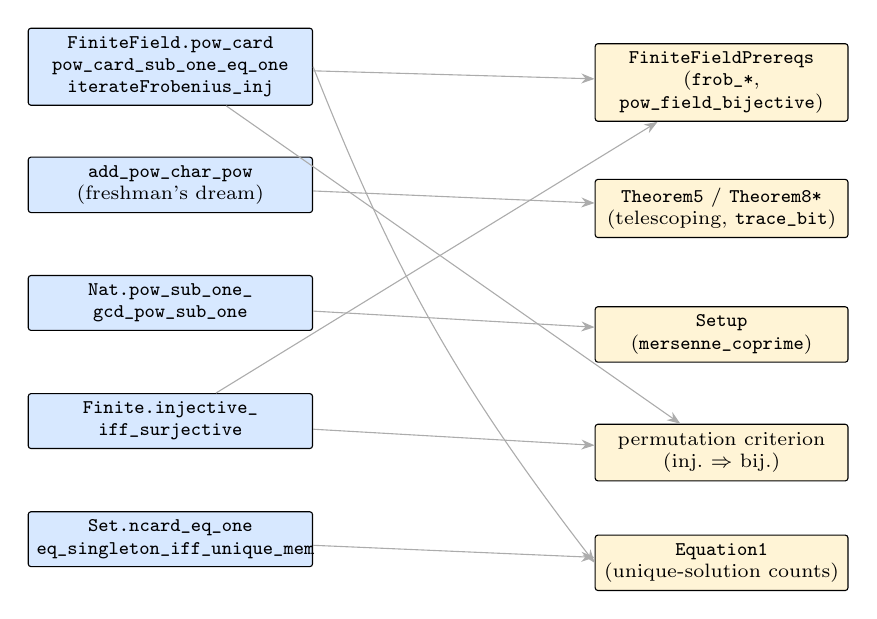
\begin{tikzpicture}[
  >=Stealth,
  found/.style={draw, rounded corners=1pt, fill=mathlibcol, font=\scriptsize,
                align=center, inner sep=3pt, text width=3.4cm},
  mod/.style={draw, rounded corners=1pt, fill=enginecol, font=\scriptsize,
              align=center, inner sep=3pt, text width=3.0cm},
  e/.style={->, gray!65},
]
\node[found] (a) at (0,0)   {\lc{FiniteField.pow_card}\\ \lc{pow_card_sub_one_eq_one}\\ \lc{iterateFrobenius_inj}};
\node[found] (b) at (0,-1.5){\lc{add_pow_char_pow}\\(freshman's dream)};
\node[found] (c) at (0,-3.0){\lc{Nat.pow_sub_one_}\\\lc{gcd_pow_sub_one}};
\node[found] (d) at (0,-4.5){\lc{Finite.injective_}\\\lc{iff_surjective}};
\node[found] (e) at (0,-6.0){\lc{Set.ncard_eq_one}\\ \lc{eq_singleton_iff_unique_mem}};

\node[mod] (m1) at (7,-0.2){\lc{FiniteFieldPrereqs}\\ (\lc{frob_*}, \lc{pow_field_bijective})};
\node[mod] (m2) at (7,-1.8){\lc{Theorem5} / \lc{Theorem8*}\\ (telescoping, \lc{trace_bit})};
\node[mod] (m3) at (7,-3.4){\lc{Setup}\\ (\lc{mersenne_coprime})};
\node[mod] (m4) at (7,-4.9){permutation criterion\\ (inj.\ $\Rightarrow$ bij.)};
\node[mod] (m5) at (7,-6.3){\lc{Equation1}\\ (unique-solution counts)};

\draw[e] (a) -- (m1);  \draw[e] (a) -- (m4);
\draw[e] (b) -- (m2);
\draw[e] (c) -- (m3);
\draw[e] (d) -- (m4); \draw[e] (d) -- (m1);
\draw[e] (e) -- (m5);
\draw[e] (a.east) to[bend right=8] (m5.west);
\end{tikzpicture}
}
\caption{The non-trivial Mathlib foundations (left) and the library layers that
consume them (right). Elementary \lc{Nat} arithmetic and general automation
(\lc{ring}, \lc{grind}, \lc{decide}, \lc{simp}, \lc{omega}) sit underneath all
of these.}
\label{fig:foundations}
\end{figure}

\clearpage

% ===========================================================================
\section{Layer 1a --- \texttt{Defs}: the pure definitions}
% ===========================================================================

The bottom of the DAG is a single Mathlib-only file of definitions.  It fixes
the ambient field and transcribes the paper's objects.

\begin{paperquote}{p.~134, standing assumptions and $q_\alpha$}
We always assume $\gcd(k,n)=1,\ k<n,\ k'\equiv 1/k \pmod n$. For
$\alpha=0,1$ we define the polynomials
\[
  q_\alpha(z)=\frac{\sum_{i=1}^{k'} z^{2^{ik}}+\alpha\,\mathrm{Tr}(z)}{z^{2^k+1}},
\]
where $\mathrm{Tr}$ denotes the trace function from $\mathbb{F}_{2^n}$ onto
$\mathbb{F}_2$. (To be formally more precise, we get a polynomial $q_\alpha$ for
each $L=\mathbb{F}_{2^n}$ if we substitute $1/z^{2^k+1}$ by
$z^{(2^n-1)-(2^k+1)}$.) We call $q_\alpha$ a generalized Kasami polynomial.
\end{paperquote}

The library realises $L=\mathbb{F}_{2^n}$ abstractly as any finite field of
characteristic $2$, and the ``$0/0=0$'' convention as the honest power
$z^{(2^n-1)-(2^k+1)}$.

\begin{lstlisting}
variable {L : Type*} [Field L] [Fintype L] [CharP L 2]

/-- The absolute trace `Tr(x) = ∑_{i<n} x^{2^i}`. -/
def Tr (n : ℕ) (x : L) : L := ∑ i ∈ Finset.range n, x ^ (2 ^ i)

/-- The generalized Kasami polynomial `q_α` (with `0/0 = 0`). -/
def qKasami (n k k' : ℕ) (α : ℕ) (z : L) : L :=
  ((∑ i ∈ Finset.Icc 1 k', z ^ (2 ^ (i * k))) + (α : L) * Tr n z)
    * z ^ (2 ^ n - 1 - (2 ^ k + 1))

/-- Equation (1): `q_α(x) = c` cleared of denominators. -/
def eqn1 (n k k' : ℕ) (α : ℕ) (c x : L) : Prop :=
  c * x ^ (2 ^ k + 1) = (∑ i ∈ Finset.Icc 1 k', x ^ (2 ^ (i * k))) + (α : L) * Tr n x
\end{lstlisting}

The auxiliary polynomials of equation~(2) are defined here too:

\begin{lstlisting}
/-- `ell(x) = c^{2^k}·x^{2^{2k}} + x^{2^k} + c·x + 1`  (equation (2)). -/
def ell (k : ℕ) (c x : L) : L :=
  c ^ (2 ^ k) * x ^ (2 ^ (2 * k)) + x ^ (2 ^ k) + c * x + 1
/-- Homogeneous part `ell0(x) = ell(x) + 1`. -/
def ell0 (k : ℕ) (c x : L) : L := ell (L := L) k c x + 1
/-- `Q(x) = c·x^{2^k} + γ²·x + γ`   (Case 2). -/
def Qmap (k : ℕ) (c γ x : L) : L := c * x ^ (2 ^ k) + γ ^ 2 * x + γ
\end{lstlisting}

% ===========================================================================
\section{Layer 1b --- \texttt{FiniteFieldPrereqs}: the finite-field engine}
% ===========================================================================

Parallel to \lc{Defs}, and also resting only on Mathlib, is the finite-field
engine.  It packages the two devices the whole proof runs on: the
\emph{Frobenius map as a bijection}, and the \emph{truncated trace}
$L(x)=\sum_{i<m}x^{2^i}$ with its additivity and Artin--Schreier telescoping.

\begin{lstlisting}
lemma frob_cycle (x : F) : x ^ Fintype.card F = x := FiniteField.pow_card x

lemma frob_bijective (r : ℕ) : Function.Bijective (fun x : F => x ^ (p ^ r)) :=
  ⟨iterateFrobenius_inj F p r,
   (Finite.injective_iff_surjective).mp (iterateFrobenius_inj F p r)⟩

/-- `x ↦ xᵃ` is a bijection when `gcd(|F|-1, a) = 1`. -/
lemma pow_field_bijective {a : ℕ} (ha : Nat.Coprime (Fintype.card F - 1) a)
    (ha_pos : 0 < a) : Function.Bijective (fun x : F => x ^ a)

/-- The truncated trace `L(x) = ∑_{i<m} x^{2^i}`. -/
def truncTrace (m : ℕ) (x : F) : F := ∑ i ∈ Finset.range m, x ^ (2 ^ i)

/-- Additivity of `L` (freshman's dream, char 2). -/
lemma truncTrace_add (m : ℕ) (x y : F) :
    truncTrace m (x + y) = truncTrace m x + truncTrace m y

/-- Artin–Schreier telescoping: `L(x)² + L(x) = x^{2^m} + x`. -/
lemma truncTrace_sq_add_self (m : ℕ) (x : F) :
    truncTrace m x ^ 2 + truncTrace m x = x ^ (2 ^ m) + x
\end{lstlisting}

The additivity of $L$ is exactly the ``freshman's dream'' $ (x+y)^{2^i}=x^{2^i}+y^{2^i}$
summed over $i$, and the telescoping identity is the algebraic heart of every
trace computation downstream.  Diagrammatically:

\begin{figure}[h]
\centering
\begin{tikzcd}[column sep=large, row sep=large]
F \times F \arrow[r, "+"] \arrow[d, "L\times L"'] & F \arrow[d, "L"] \\
F \times F \arrow[r, "+"'] & F
\end{tikzcd}
\qquad\qquad
\begin{tikzcd}[column sep=huge]
x \arrow[r, "L"] \arrow[d, "{(\,\cdot\,)^2+\,\cdot\,}"']
   & L(x) \arrow[d, "{(\,\cdot\,)^2+\,\cdot\,}"] \\
x^{2^m}+x & L(x)^2+L(x) \arrow[l, equal]
\end{tikzcd}
\caption{Left: additivity of the truncated trace (\lc{truncTrace_add}).
Right: the Artin--Schreier telescoping (\lc{truncTrace_sq_add_self}).}
\end{figure}

% ===========================================================================
\section{Layer 2a --- \texttt{Setup}: the elementary opening of the proof}
% ===========================================================================

This module is the engine-free opening of Theorem~1's proof --- everything
\emph{before} equations (1)/(2).

\begin{paperquote}{p.~135, opening of the proof of Theorem 1}
\emph{Proof.} First note that $(2^k-1)^{-1}\pmod{2^n-1}$ exists, since
$\gcd(k,n)=1$. We have $q_\alpha(0)=0$, using the convention ``$0/0=0$''. To
verify the ``only if'' part, observe that $k'+\alpha n\equiv 0\pmod 2$ is
equivalent to $q_\alpha(1)=k'\cdot 1+\alpha\cdot\mathrm{Tr}(1)=0$.
\end{paperquote}

Each sentence maps to one declaration.  The existence of the modular inverse
reduces to the Mersenne-gcd fact
$\gcd(2^k-1,2^n-1)=2^{\gcd(k,n)}-1$:

\begin{lstlisting}
theorem mersenne_coprime (h : Nat.Coprime k n) :
    Nat.Coprime (2 ^ k - 1) (2 ^ n - 1) := by
  unfold Nat.Coprime at *; rw [Nat.pow_sub_one_gcd_pow_sub_one]; simp [h]

theorem inv_mod_exists (h : Nat.Coprime k n) (hn : 1 < 2 ^ n - 1) :
    ∃ b, (2 ^ k - 1) * b % (2 ^ n - 1) = 1

theorem qKasami_zero (α : ℕ) : qKasami (L := L) n k k' α 0 = 0

theorem qKasami_one (α : ℕ) :
    qKasami (L := L) n k k' α 1 = ((k' + α * n : ℕ) : L)

/-- The "only if" part at the value q_α(1). -/
theorem qKasami_one_eq_zero_iff (α : ℕ) :
    qKasami (L := L) n k k' α 1 = 0 ↔ (k' + α * n) % 2 = 0
\end{lstlisting}

% ===========================================================================
\section{Layer 2b --- \texttt{Theorem5}: the trace-free permutation criterion}
% ===========================================================================

This is the $\alpha=0$ backbone and the source of the three reduction lemmas
reused by the equation-(1) thread.  Dobbertin's Theorem~5 treats the
\emph{trace-free} polynomial $q^{(\varepsilon)}$, and its proof \emph{is} the
root-count argument that Theorem~1 quotes.

\begin{paperquote}{p.~135, the reduction to the linearised equation}
To prove the ``if'' part assume $k'+\alpha n\equiv 1\pmod 2$. We shall show
that for each fixed $c\in L$, the equation
\[ c\,x^{2^k+1}=\sum_{i=1}^{k'}x^{2^{ik}}+\alpha\,\mathrm{Tr}(x) \tag{1}\]
has at most one solution in $L$. Adding the $2^k$-th power of this equation to
itself we get $\ldots$ and consequently
\[ \ell(x)=c^{2^k}x^{2^{2k}}+x^{2^k}+cx+1=0. \tag{2}\]
\end{paperquote}

The module first sets up the step-$2^k$ partial trace $P(x)=\sum_{j<k'}x^{2^{jk}}$
and the numerator sum $S(x)=\sum_{i=1}^{k'}x^{2^{ik}}$, with $S=P^{2^k}$ and the
telescoping $P^{2^k}+P=x^2+x$ (via \lc{pTrace_telescope}).  The (1)$\Rightarrow$(2)
reduction is then packaged as \lc{ell_of_eq}:

\begin{lstlisting}
noncomputable def pTrace (k k' : ℕ) (x : F) : F := ∑ j ∈ Finset.range k', x ^ (2 ^ (j * k))
noncomputable def sTrace (k k' : ℕ) (x : F) : F := ∑ i ∈ Finset.Icc 1 k', x ^ (2 ^ (i * k))
noncomputable def qeps (n k k' : ℕ) (ε : F) (x : F) : F :=
  (sTrace k k' x + ε) * x ^ (2 ^ n - 1 - (2 ^ k + 1))

/-- (1) => (2): on units, `q^{(ε)}(x) = c` gives `ell(x) = 0`. -/
lemma ell_of_eq (hn : Fintype.card F = 2 ^ n) (hkk' : k * k' % n = 1)
    (hε : ε = 0 ∨ ε = 1) (hx : x ≠ 0) (hex : sTrace k k' x + ε = c * x ^ (2 ^ k + 1)) :
    c ^ (2 ^ k) * x ^ (2 ^ (2 * k)) + x ^ (2 ^ k) + c * x + 1 = 0
\end{lstlisting}

The two case lemmas of Theorem~1 also live here, in their trace-free form:

\begin{lstlisting}
/-- Case 1: a nonzero root of ell0 forces `c` into the image of `γ ↦ γ^{2^k+1}+γ`. -/
lemma ell0_root_imp_image (hn : Fintype.card F = 2 ^ n) (hk : 0 < k) (hkn : k < n)
    (hc : c ≠ 0) (ht : t ≠ 0)
    (h0 : c ^ (2 ^ k) * t ^ (2 ^ (2 * k)) + t ^ (2 ^ k) + c * t = 0) :
    ∃ γ : F, c = γ ^ (2 ^ k + 1) + γ

/-- Case 2: the factorisation `ell = Q^{2^k} + f·Q` with `f = γ^{2^k-1}+γ⁻¹`. -/
lemma Q_factor (hγ : γ ≠ 0) (hcdef : c = γ ^ (2 ^ k + 1) + γ) (t : F) :
    c ^ (2 ^ k) * t ^ (2 ^ (2 * k)) + t ^ (2 ^ k) + c * t + 1
      = (qPoly γ c k t) ^ (2 ^ k) + (γ ^ (2 ^ k - 1) + γ⁻¹) * (qPoly γ c k t)
\end{lstlisting}

Culminating in the trace-free criterion:

\begin{lstlisting}
/-- Theorem 5: `q^{(ε)}` is a permutation of `F` iff `ε ≡ k'+1 (mod 2)`. -/
theorem theorem_5 (hn : Fintype.card F = 2 ^ n) (hk : 0 < k) (hkn : k < n)
    (hcop : Nat.Coprime k n) (hkk' : k * k' % n = 1) (hexp : 2 ^ k + 1 < 2 ^ n - 1)
    (hε : ε = 0 ∨ ε = 1) :
    Function.Bijective (qeps n k k' ε) ↔ (ε = 1 ↔ Even k')
\end{lstlisting}

The internal logic of the reduction $(1)\Rightarrow(2)$ is the following
computation, which is exactly what \lc{ell_of_eq} encodes:

\begin{figure}[h]
\centering
\begin{tikzcd}[column sep=1.9cm, row sep=1.1cm]
\textbf{(1)}\ S(x)+\varepsilon = c\,x^{2^k+1}
   \arrow[r, "P^{2^k}=S"] \arrow[d, "P^{2^k}+P=x^2+x"']
 & P = c\,x^{2^k+1}+x^2+x+\varepsilon
   \arrow[d, "(\,\cdot\,)^{2^k}"] \\
S = P^{2^k}
   \arrow[r, "\varepsilon^{2^k}=\varepsilon"']
 & c^{2^k}x^{2^{2k}}+x^{2^k}+c\,x+1 = 0\ \ \textbf{(2)}
\end{tikzcd}
\caption{The telescoping computation behind \lc{ell_of_eq}: substitute
$P=(x^2+x)+S$, raise to the $2^k$ power, divide by $x^{2^k}$.}
\end{figure}

% ===========================================================================
\section{Layer 2c --- \texttt{Theorem8Trace}: the two trace identities}
% ===========================================================================

The $\alpha=1$ branch needs two facts about the absolute trace, isolated here.

\begin{lstlisting}
/-- Frobenius-invariance: `Tr(x^{2^k}) = Tr(x)`. -/
theorem trace_frob_shift (hn : Fintype.card F = 2 ^ n) (k : ℕ) (x : F) :
    truncTrace n (x ^ (2 ^ k)) = truncTrace n x

/-- Artin–Schreier vanishing: `Tr(t^{2^k} + t) = 0`. -/
theorem trace_artin_schreier_zero (hn : Fintype.card F = 2 ^ n) (k : ℕ) (t : F) :
    truncTrace n (t ^ (2 ^ k) + t) = 0
\end{lstlisting}

\begin{figure}[h]
\centering
\begin{tikzcd}[column sep=huge]
t \arrow[r, "{x\,\mapsto\, x^{2^k}+x}"] \arrow[dr, "\mathrm{Tr}(\,\cdot\,)=0"'] & t^{2^k}+t \arrow[d, "\mathrm{Tr}"] \\
 & 0
\end{tikzcd}
\caption{\lc{trace_artin_schreier_zero} as the composite
$\mathrm{Tr}\circ(x\mapsto x^{2^k}+x)=0$, using
$\mathrm{Tr}(x^{2^k})=\mathrm{Tr}(x)$ (\lc{trace_frob_shift}) and additivity.}
\end{figure}

% ===========================================================================
\section{Layer 3a --- \texttt{Theorem8C1}: $\mathrm{Tr}(x)\in\{0,1\}$ and \texttt{gmap}}
% ===========================================================================

Building on \lc{Theorem5} and the prerequisites, this file proves the trace is a
\emph{bit} and defines the trace-version Kasami map.

\begin{lstlisting}
/-- `Tr(x)² = Tr(x)`. -/
theorem trace_sq (hn : Fintype.card F = 2 ^ n) (x : F) :
    (truncTrace n x) ^ 2 = truncTrace n x
/-- `Tr(x) ∈ {0,1}`. -/
theorem trace_bit (hn : Fintype.card F = 2 ^ n) (x : F) :
    truncTrace n x = 0 ∨ truncTrace n x = 1
/-- The trace version `g(x) = q^{(Tr x)}(x)`. -/
noncomputable def gmap (n k kk : ℕ) (x : F) : F := qeps n k kk (truncTrace n x) x
\end{lstlisting}

\lc{trace_sq} is an immediate consequence of the telescoping identity together
with Fermat ($x^{2^n}=x$): $\mathrm{Tr}(x)^2+\mathrm{Tr}(x)=x^{2^n}+x=0$, whence
$\mathrm{Tr}(x)\in\{0,1\}$ because $t^2=t$ has only the roots $0,1$ in a field.

% ===========================================================================
\section{Layer 3b --- \texttt{Q1General}: the $\alpha=1$ criterion}
% ===========================================================================

The trace-version analogue of \lc{theorem_5}, i.e.\ the $\alpha=1$ backbone:

\begin{lstlisting}
/-- The `α = 1` criterion: `g = gmap` is a permutation iff `kk + n` is odd. -/
theorem gmap_bijective_iff (hn : Fintype.card F = 2 ^ n) (hk : 0 < k) (hkn : k < n)
    (hcop : Nat.Coprime k n) (hkk' : k * kk % n = 1) (hexp : 2 ^ k + 1 < 2 ^ n - 1) :
    Function.Bijective (Thm8C1.gmap (F := F) n k kk) ↔ Odd (kk + n)
\end{lstlisting}

% ===========================================================================
\section{Layer 4 --- \texttt{Equation1}: the headline thread}
% ===========================================================================

The top of the DAG glues everything together.  Three \emph{bridge} lemmas
identify the paper's $q_\alpha$ (\lc{qKasami}) with the two library backbones,
after which Theorem~1 is a two-case dispatch.

\subsection{Bridges: \texttt{qKasami} $\leftrightarrow$ \texttt{qeps} / \texttt{gmap}}

\begin{lstlisting}
lemma qKasami_zero_eq_qeps (z : L) :
    qKasami (L := L) n k k' 0 z = Dobbertin.Thm5.qeps n k k' (0 : L) z
lemma qKasami_one_eq_gmap (z : L) :
    qKasami (L := L) n k k' 1 z = Dobbertin.Thm8C1.gmap n k k' z
lemma qKasami_mul_unit (hn : Fintype.card L = 2 ^ n) (hexp : 2 ^ k + 1 ≤ 2 ^ n - 1)
    (α : ℕ) (hx : x ≠ 0) :
    qKasami (L := L) n k k' α x * x ^ (2 ^ k + 1)
      = (∑ i ∈ Finset.Icc 1 k', x ^ (2 ^ (i * k))) + (α : L) * Tr n x
\end{lstlisting}

\begin{figure}[h]
\centering
{\footnotesize
\begin{tikzcd}[column sep=1.15cm, row sep=1.0cm]
 & \lc{qKasami}\ (=q_\alpha)
   \arrow[dl, "\alpha=0"'] \arrow[dr, "\alpha=1"] & \\
\lc{Thm5.qeps}\ (q^{(0)})
   \arrow[d, "\lc{theorem_5}"'] & &
\lc{Thm8C1.gmap}\ (g=q^{(\mathrm{Tr})})
   \arrow[d, "\lc{gmap_bijective_iff}"] \\
\big(\text{bij.}\ \Leftrightarrow\ k'\ \text{odd}\big)
   \arrow[dr, Rightarrow] & &
\big(\text{bij.}\ \Leftrightarrow\ k'{+}n\ \text{odd}\big)
   \arrow[dl, Rightarrow] \\
 & \lc{theorem_1}:\ \text{bij.}\ \Leftrightarrow\ (k'+\alpha n)\bmod 2 = 1 &
\end{tikzcd}
}
\caption{Assembly of \lc{theorem_1}: the bridges (\lc{qKasami_zero_eq_qeps},
\lc{qKasami_one_eq_gmap}) reduce the two parities to \lc{theorem_5} ($\alpha=0$)
and \lc{gmap_bijective_iff} ($\alpha=1$).}
\end{figure}

\subsection{Theorem 1}

\begin{paperquote}{p.~135--136, statement of Theorem 1}
\textbf{Theorem 1.} A generalized Kasami polynomial $q_\alpha$ is a permutation
polynomial on $L$ if and only if $k'+\alpha n\equiv 1\pmod 2$. That is,
$q_0$ is a permutation polynomial if and only if $k'$ is odd;
$q_1$ is a permutation polynomial if and only if $n\equiv k'+1\pmod 2$.
\end{paperquote}

\begin{lstlisting}
theorem theorem_1 (hn : Fintype.card L = 2 ^ n) (hk : k < n) (hcop : Nat.Coprime k n)
    (hk' : k * k' % n = 1 % n) (hk0 : 0 < k) (hexp : 2 ^ k + 1 < 2 ^ n - 1)
    (α : ℕ) (hα : α = 0 ∨ α = 1) :
    Function.Bijective (qKasami (L := L) n k k' α) ↔ (k' + α * n) % 2 = 1
\end{lstlisting}

\subsection{The step (1) $\Rightarrow$ (2)}

This is the first substantive step of the proof.

\begin{paperquote}{p.~135, the passage to (2)}
Adding the $2^k$-th power of this equation to itself we get $\ldots$ and
consequently $\ \ell(x)=c^{2^k}x^{2^{2k}}+x^{2^k}+cx+1=0.$ \hfill (2)
\end{paperquote}

\begin{lstlisting}
theorem eqn2_of_eqn1 (hn : Fintype.card L = 2 ^ n) (hkk1 : k * k' % n = 1)
    (α : ℕ) (c x : L) (hx : x ≠ 0) (h : eqn1 (L := L) n k k' α c x) :
    ell (L := L) k c x = 0
\end{lstlisting}

The proof feeds the numerator equation into \lc{Thm5.ell_of_eq}; the side
condition ``$\alpha\,\mathrm{Tr}(x)\in\{0,1\}$'' needed by the trace-free lemma
is exactly \lc{Thm8C1.trace_bit}.  See Correction~\ref{cor:eqn2} for why the
hypothesis \lc{hx : x ≠ 0} is present.

\subsection{The two cases}

\begin{paperquote}{p.~136, the trichotomy and Case 1}
Note that $\ell(x)=0$ if and only if
$c\,x^{2^k+1}+\sum_{i=1}^{k'}x^{2^{ik}}+\alpha\,\mathrm{Tr}(x)=0$ or $1$. As we
shall see, $\ell$ has either one, two or four roots in $L$. It will be shown that
at most one of them is a solution of (1). \\[2pt]
\textbf{Case 1.} $c\neq\gamma^{2^k+1}+\gamma$ for all $\gamma\in L$. In this
case, the homogeneous part $\ell_0(x)=\ell(x)+1$ of (2) has no non-zero
solution, since $\ell_0(x)=\tfrac1c\,(\gamma_0(x)^{2^k+1}+\gamma_0(x)+c)^2\,x$
for $\gamma_0(x)=(c\,x^{2^k-1})^{2^{n-1}}$. Hence (2) has precisely one solution,
and we are done.
\end{paperquote}

\begin{lstlisting}
theorem theorem_1_case1 (hn : Fintype.card L = 2 ^ n) (hk0 : 0 < k) (hkn : k < n)
    (c : L) (hc : ∀ γ : L, c ≠ γ ^ (2 ^ k + 1) + γ) :
    {x : L | ell (L := L) k c x = 0}.ncard = 1
\end{lstlisting}

\begin{paperquote}{p.~136, Case 2}
\textbf{Case 2.} $c=\gamma^{2^k+1}+\gamma$ for some $\gamma\in L$. Setting
$Q(x)=c\,x^{2^k}+\gamma^2 x+\gamma,\ \ f=\gamma^{2^k-1}+1/\gamma$ we have
$\ell(x)=Q(x)^{2^k}+f\,Q(x)$ and therefore $\ell(x)=0$ if and only if $Q(x)=0$
or $Q(x)=1/f\ldots$
\end{paperquote}

\begin{lstlisting}
theorem ell_eq_Q (k : ℕ) (c γ x : L) (hγ : γ ≠ 0) (hc : c = γ ^ (2 ^ k + 1) + γ) :
    ell (L := L) k c x
      = Qmap (L := L) k c γ x ^ (2 ^ k) + (γ ^ (2 ^ k - 1) + γ⁻¹) * Qmap (L := L) k c γ x

theorem theorem_1_case2 (hn : Fintype.card L = 2 ^ n) (hk : k < n)
    (hcop : Nat.Coprime k n) (hk' : k * k' % n = 1 % n) (hk0 : 0 < k)
    (hexp : 2 ^ k + 1 < 2 ^ n - 1) (α : ℕ) (hα : α = 0 ∨ α = 1)
    (hpar : (k' + α * n) % 2 = 1) (c γ : L) (hc0 : c ≠ 0) (hc : c = γ ^ (2 ^ k + 1) + γ) :
    {x : L | x ≠ 0 ∧ eqn1 (L := L) n k k' α c x}.ncard = 1
\end{lstlisting}

The whole case analysis is the tree of Figure~\ref{fig:cases}.

\begin{figure}[h]
\centering
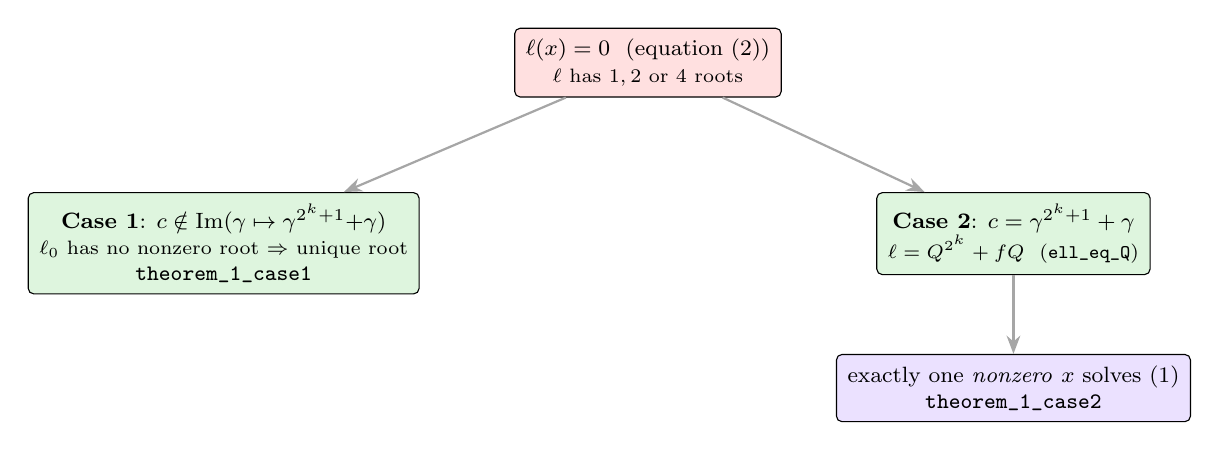
\begin{tikzpicture}[
  >=Stealth, node distance=8mm,
  n/.style={draw, rounded corners=2pt, align=center, font=\footnotesize, inner sep=4pt},
  e/.style={->, thick, gray!70},
]
\node[n, fill=headcol] (root) {$\ell(x)=0$\ \ (equation (2))\\ \scriptsize$\ell$ has $1,2$ or $4$ roots};
\node[n, fill=defscol, below left=12mm and 1.2cm of root] (c1)
  {\textbf{Case 1}: $c\notin\mathrm{Im}(\gamma\mapsto\gamma^{2^k+1}{+}\gamma)$\\
   \scriptsize $\ell_0$ has no nonzero root $\Rightarrow$ unique root\\ \lc{theorem_1_case1}};
\node[n, fill=defscol, below right=12mm and 1.2cm of root] (c2)
  {\textbf{Case 2}: $c=\gamma^{2^k+1}+\gamma$\\
   \scriptsize $\ell=Q^{2^k}+fQ$ \ (\lc{ell_eq_Q})};
\node[n, fill=bridgecol, below=10mm of c2] (c2a)
  {exactly one \emph{nonzero} $x$ solves (1)\\ \lc{theorem_1_case2}};
\draw[e] (root) -- (c1);
\draw[e] (root) -- (c2);
\draw[e] (c2) -- (c2a);
\end{tikzpicture}
\caption{The case analysis of Theorem~1's ``if'' direction: equation (1) has
at most one solution for each fixed $c$.}
\label{fig:cases}
\end{figure}

Finally, \lc{theorem_1_case2} is assembled from surjectivity of $q_\alpha$
(via \lc{theorem_1}) and the denominator-clearing bridge \lc{qKasami_mul_unit},
packaged through \lc{Set.ncard_eq_one}:

\begin{figure}[h]
\centering
\begin{tikzcd}[column sep=1.5cm, row sep=0.9cm]
\lc{theorem_1}\ (\text{surj.}) \arrow[r, "{\exists a,\ q_\alpha(a)=c}"]
  & a\neq 0 \arrow[d, "\lc{qKasami_mul_unit}"] \\
\lc{Set.ncard_eq_one} \arrow[u, "\text{unique mem}"]
  & \{x\neq 0 : \lc{eqn1}\ x\}=\{a\}
    \arrow[l, "\lc{eq_singleton_iff_unique_mem}"']
\end{tikzcd}
\caption{Assembly of \lc{theorem_1_case2}.}
\end{figure}

% ===========================================================================
\section{The two documented corrections}
% ===========================================================================

Two internal statements are minimally strengthened relative to a literal
transcription, because the library works with the polynomial-cleared form
\lc{eqn1} rather than the rational identity $q_\alpha(x)=c$. Both are documented
in-source.

\begin{correction}[\lc{eqn2_of_eqn1}]\label{cor:eqn2}
At $x=0$ the \emph{cleared} equation (1) reads $0=0$ and is vacuously true, yet
$\ell(0)=1\neq0$. So ``(1)$\Rightarrow\ell=0$'' requires $x\neq0$. This is an
artefact of clearing denominators; the paper argues about $q_\alpha(x)=c$, where
the $x=0$ case is handled separately by $q_\alpha(0)=0$.
\end{correction}

\begin{correction}[\lc{theorem_1_case2}]
$x=0$ always satisfies the cleared \lc{eqn1}, so counting \emph{all} solutions
never gives $1$. The paper's ``exactly one of the roots solves (1)'' is
faithfully the count of \emph{nonzero} solutions (requiring $c\neq0$, i.e.
$\gamma\neq1$).
\end{correction}

% ===========================================================================
\section{Alternative foundations and proof paths (summary)}
% ===========================================================================

For completeness, the accompanying \texttt{ARCHITECTURE\_AND\_ALTERNATIVES.md}
records alternative starting points. In brief:
\begin{itemize}[nosep]
  \item \textbf{Field object:} abstract \lc{[Field L][Fintype L][CharP L 2]} with
    \lc{card L = 2^n} (current) vs.\ Mathlib's \lc{GaloisField 2 n} (removes the
    cardinality-hypothesis threading).
  \item \textbf{Trace:} the bespoke \lc{truncTrace} (current, \lc{ring}-friendly)
    vs.\ Mathlib's \lc{Algebra.trace} (connects to the general theory, at the
    cost of an identification proof).
  \item \textbf{Permutation criterion:} explicit root-counting (current, mirrors
    the paper) vs.\ the $\mathbb{F}_2$-linear-kernel / rank--nullity view
    (\lc{LinearMap.injective_iff_surjective}) vs.\ \lc{Polynomial} degree bounds.
  \item \textbf{Step (1)$\Rightarrow$(2):} the \lc{Thm5.ell_of_eq} telescoping
    (current) vs.\ a direct Frobenius-additive \lc{ring}/\lc{linear_combination}
    computation.
\end{itemize}

\end{document}
